\chapter{The Frontend Application}
\label{frontend}
	\section{Introduction}
		\begin{figure}[H]
			\iftrue
			\caption{Frontend Application}
			\centering
			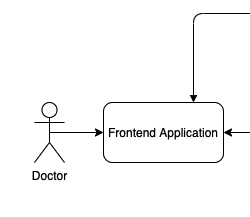
\includegraphics[scale=0.5]{figures/frontend}
			\fi
		\end{figure}
		This chapter will look at the technology stack, internals, and points of interest of the frontend application. The frontend application's 
		purpose is to serve as a visual middleware between the end-user (The Doctor) and the system itself. It  propagates the actions of the user 
		into the system by using plain HTTPS Requests, via a stateful[\cite{session-rfc6265}], Json-based[\cite{json-rfc7159}] Https[\cite{rfc2818}]
		RESTFull[\cite{restful-rfc7231}] protocol (for more information, please see chapter \ref{API}).
	\section{Technology Stack}
		The Frontend application uses the following frameworks and libraries
		\begin{itemize}
			\item React v18.0
			\item Boostrap v4
			\item Axios Requests
			\item Hansontable v8.3.2
		\end{itemize}
		\subsection{React}
			React.js is an open-source javascript framework for developing frontend applications. It is created by Facebook and maintained 
			by the open-source community as well as from some individual companies. It encourages the creation of applications with 
			well-defined state and state transitions by composing lightweight and reusable UI Elements called 'Components.' The system's 
			behavior is modeled strictly by events generated due to a state transition, and the components should act accordingly. 
			Our Frontend Application contains 16 independent components that communicate with each other by callbacks. An exhaustive 
			list of the components is given below.
			\begin{center}
				\begin{tabular}{ |c|c| } 
					\hline
					Body & The entry-point application-wide component \\
					About & The About page \\
					Home & The Home Page \\
					Hints & The Instruction manual at home page \\
					Login & The login form \\
					MyPatients & The patients list \\
					MyScans & The scan list \\
					NewPatient & The new patient form \\
					NewScan & The new scan form \\
					Notifications & The notifications list \\
					PatientView & The patiet's detailed view \\
					ScanView & The scan's detailed view \\
					Profile & The users profile page \\
					Nav & The Navigation Bar \\
					Alert & The Alert message box\\
					Content& Main view and Action bar\\
					\hline
				\end{tabular}
			\end{center}
			An example screen with its respective components highlighted is shown below...
			\begin{figure}[H]
				\iftrue
				\caption{React Components on example screen}
				\centering
				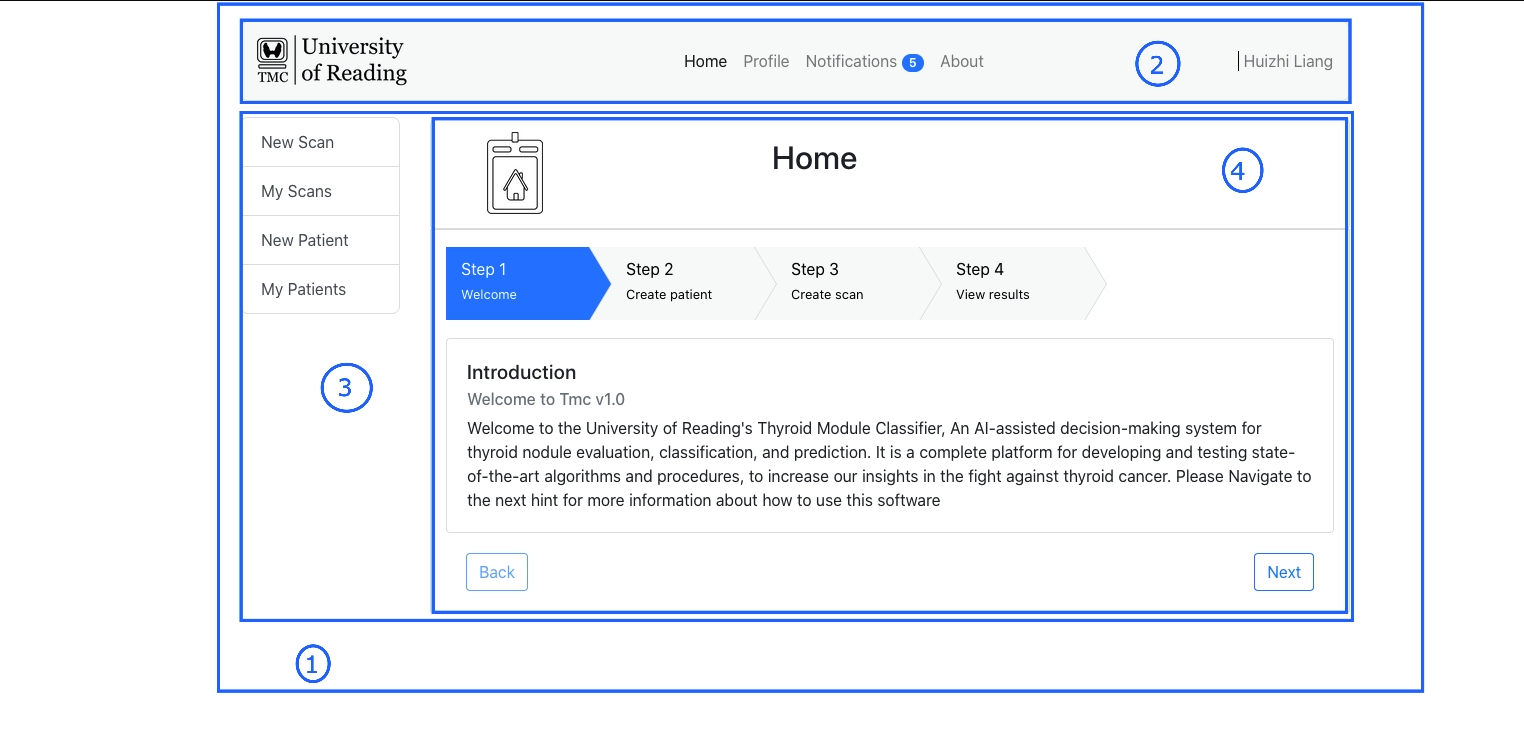
\includegraphics[scale=0.3]{figures/react-components-example}
				\fi
			\end{figure}
			...where the marked areas are ascosiated on the respective components based on the mappings below.
			\begin{center}
				\begin{tabular}{ |c|c| } 
					\hline
					1 & Body \\
					2 & NavBar \\
					3 & Content \\
					4 & Hints \\
					\hline
				\end{tabular}
			\end{center}
		\subsection{Boostrap}
			Bootstrap is an open-source CSS and Javascript web development network. It contains web templates, as well as forms, 
			buttons, and navigation elements. Boostrap is used extensively throughout the frontend application to enable a user-friendly 
			experience and cross-compatibility to various browsers and mobile devices.
			\begin{figure}[H]
				\centering
				\begin{subfigure}[b]{0.45\linewidth}
					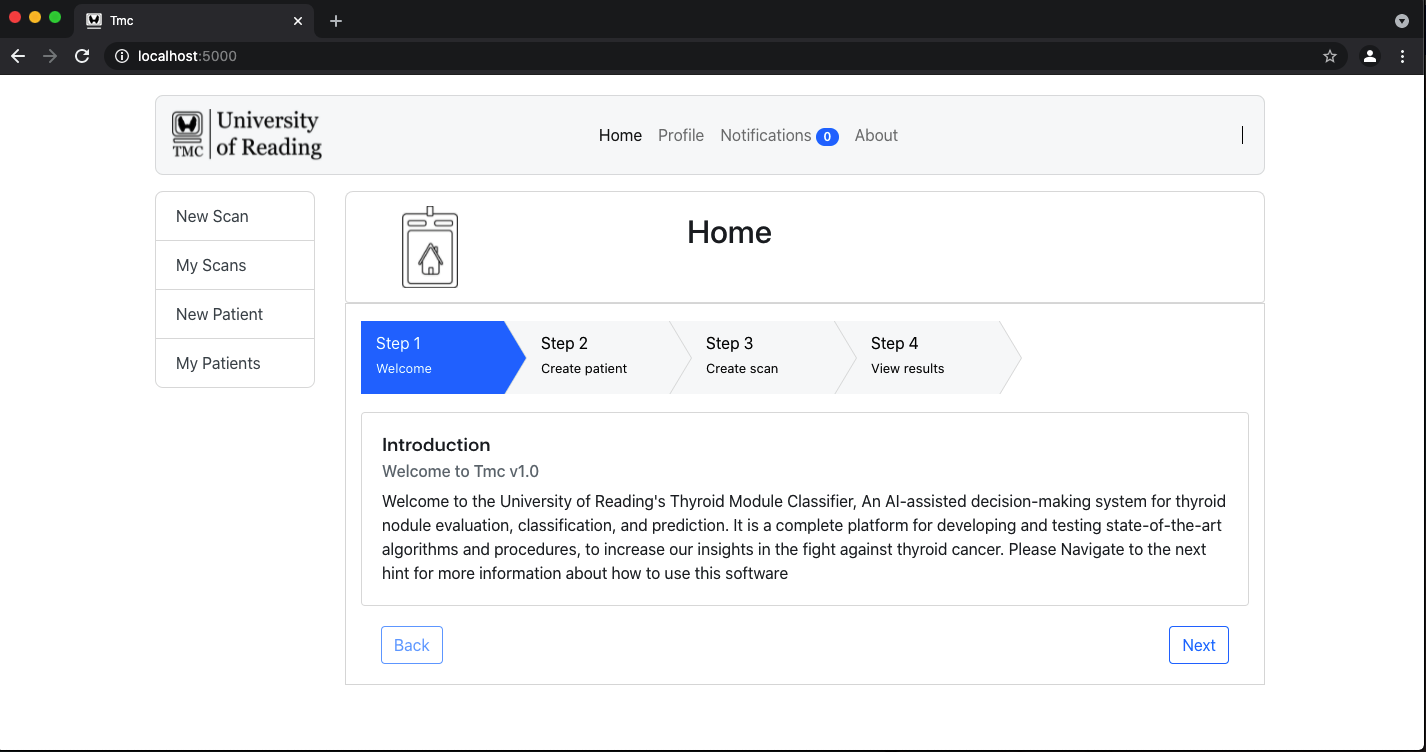
\includegraphics[width=\linewidth]{figures/tmc-runs-chrome}
					\caption{System Works on Chrome}\label{fig:mouse}
				\end{subfigure}
				
				\begin{subfigure}[b]{0.45\linewidth}
					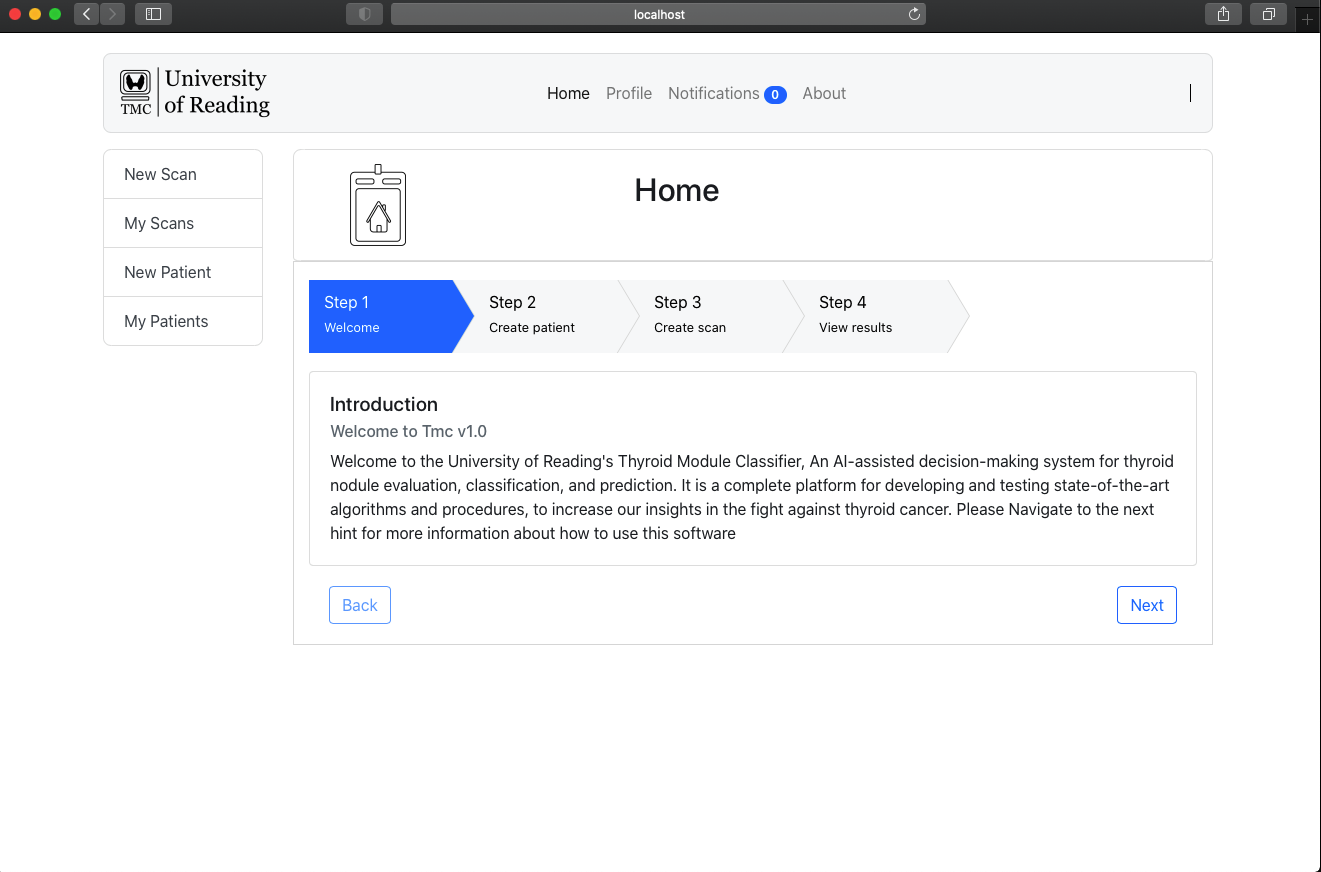
\includegraphics[width=\linewidth]{figures/tmc-runs-safari}
					\caption{System Works on Safari}\label{fig:gull}
				\end{subfigure}
				\begin{subfigure}[b]{0.45\linewidth}
					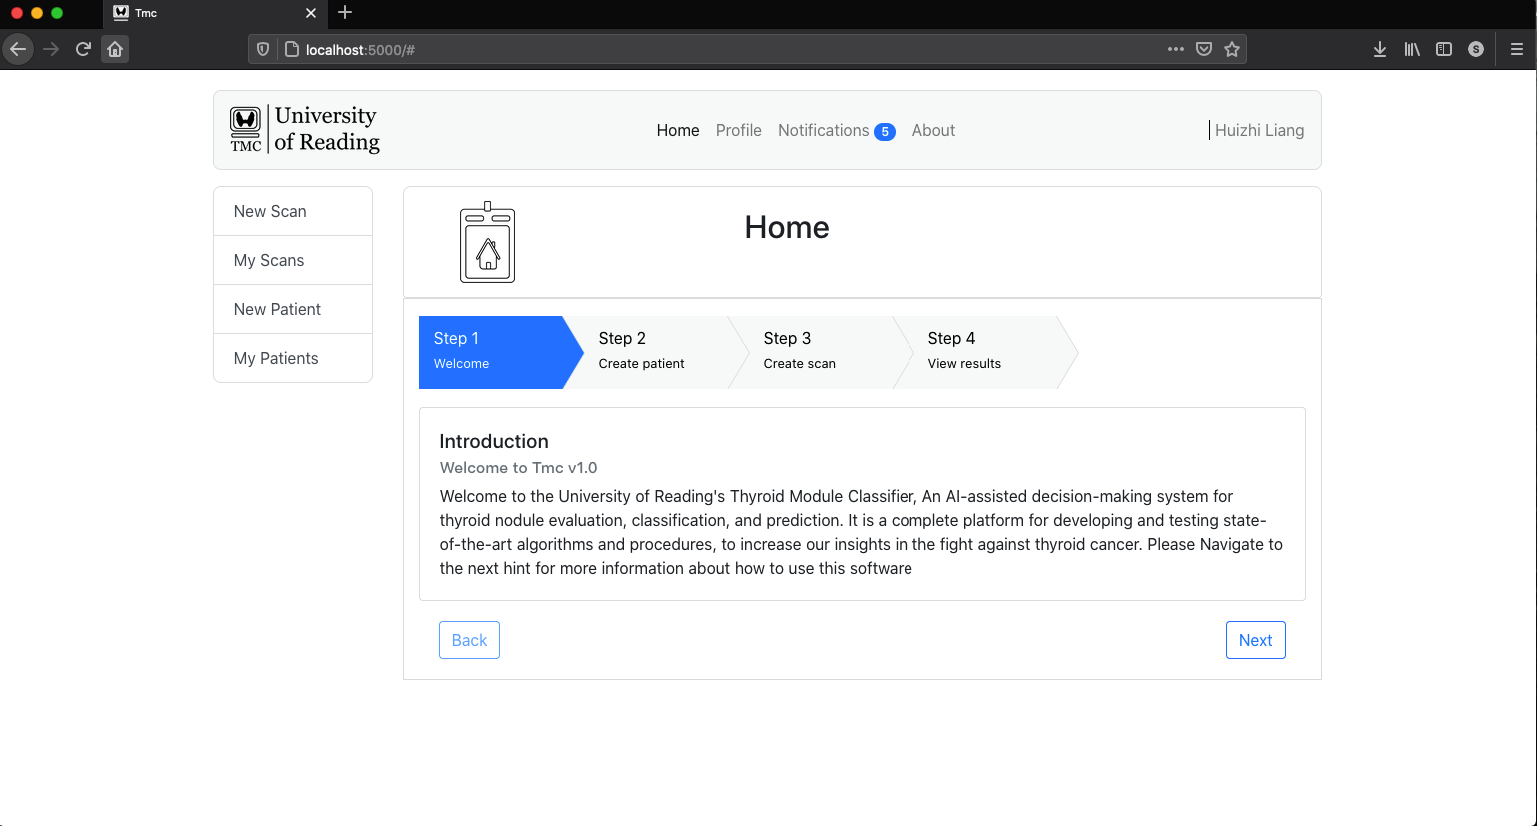
\includegraphics[width=\linewidth]{figures/tmc-runs-firefox}
					\caption{System Works on Firefox}\label{fig:tiger}
				\end{subfigure}
				\caption{Boostrap runs consistetly everywhere}
				\label{fig:animals}
			\end{figure}
		\subsection{Axios Requests}
			'Axios is a popular, promise-based HTTP client that sports an easy-to-use API and can be used in both the browser and 
			Node.js.'[\cite{jacques_2018}]. Axios enables the communication of the Frontend Application with the Backend Services; 
			it does this asynchronously, so it does not block the main thread of  execution; this feature enables the application to 
			be as smooth and responsive as possible, even under heavy loads(If the backend services are not responding fast enough, 
			functionality not needed the request responce is not affected.)
		\subsection{Hansontable}
			Hansontable is a javascript library providing a fully functional MS Excel-style spreadsheet for generic use. We use this spreadsheet on two 
			components, MyPatients and MyScans.
			\begin{figure}[H]
				\iftrue
				\caption{Hansontable example with the first two lines selected}
				\centering
				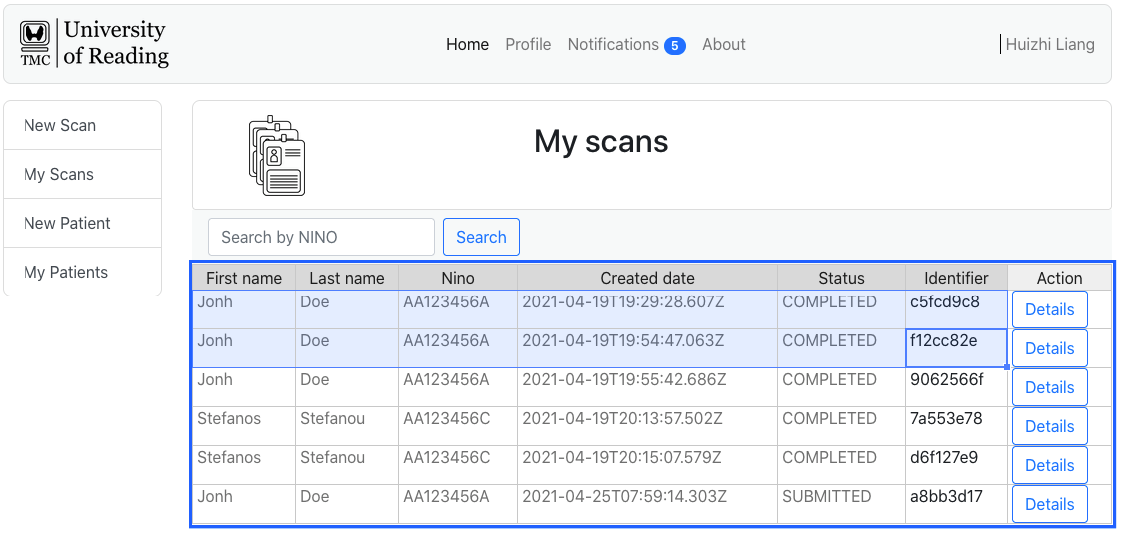
\includegraphics[scale=0.3]{figures/hansontable-example}
				\fi
			\end{figure}
			
			
			
			